\documentclass[../../../../main.tex]{subfiles}
\begin{document}
\section*{京都大学 1981年 前期}
\begin{center}
\begin{tabular}{|c|c|c|c|c|}
\hline
 & & 思 & 計 & 総 \\ \hline
[1] & 多変数 & B & C & B $\star$ \\ \hline
[2] & ベクトル & B & A & B \\ \hline
[3] & 多変数 & B & B & B \\ \hline
[4] & 多変数 & B & B & B \\ \hline
[5] & 場合の数 & B & B & B \\ \hline
[6] & 不等式 & C & B & C $\star$ \\ \hline
\end{tabular}
\end{center}

\subsection*{第1問}
[解答] 題意の直線$\ell$は$y$軸と平行でないので、その傾きを$m$とする。$\ell$と$y=\frac{1}{4}x^2$の交点の$x$座標を$\left(\alpha, \frac{1}{4}\alpha^2\right)$, $\left(\beta, \frac{1}{4}\beta^2\right)$とおく。($\alpha < \beta$)
ここで、$\ell : y = m(x-4)+5$ だから、$\alpha, \beta$は次の2次方程式
\[ \frac{1}{4}x^2 - m(x-4) - 5 = 0 \cdots \text{①} \]
の2解である。(図形的に2解持つことは明らかである) $|PQ|^2$ を $f(m)$ とおく。
\[ f(m) = (\beta - \alpha)^2 + \left( \frac{1}{4}\beta^2 - \frac{1}{4}\alpha^2 \right)^2 = \left( 1 + \frac{1}{16}(\beta + \alpha)^2 \right)(\beta - \alpha)^2 \cdots \text{②} \]
①から、
\begin{align*}
\alpha + \beta &= 4m \\
\beta - \alpha &= 2 \sqrt{(2m)^2 - 16m + 20} \quad (\because \beta > \alpha) \\
&= 4 \sqrt{m^2 - 4m + 5}
\end{align*}
だから、②に代入して
\begin{align*}
f(m) &= \left\{ 1 + \frac{1}{16}(4m)^2 \right\} 16(m^2 - 4m + 5) \\
&= 16(1+m^2)(m^2 - 4m + 5)
\end{align*}
この$\min$を求める。
\begin{align*}
f'(m) &= 16 \left[ 2m(m^2-4m+5) + (1+m^2)(2m-4) \right] \\
&= 16 \left[ 4m^3 - 12m^2 + 12m - 4 \right] \\
&= 64 (m-1)^3
\end{align*}
よって下表をうる。

\begin{center}
\begin{tabular}{|c|c|c|c|}
\hline
$m$ & $\cdots$ & $1$ & $\cdots$ \\ \hline
$f'$ & $-$ & $0$ & $+$ \\ \hline
$f$ & $\searrow$ & & $\nearrow$ \\ \hline
\end{tabular}
\end{center}

$|PQ| \ge 0$ より、$|PQ|^2$ が$\min$のとき $|PQ|$ も$\min$であることから、もとめるカタムキは$1$である。

\subsection*{第2問}
[解] 点$X$に対し $\overrightarrow{OX} = \vec{x}$とすると
$\vec{a}, \vec{b}, \vec{c}$ は1次独立であり $\cdots \text{①}$
\begin{align*}
\vec{p_1} &= k\vec{a} \\
\vec{p_2} &= l\vec{a} + (1-l)\vec{b} \\
\vec{p_3} &= (1-m)\vec{b} + m\vec{c} \\
\vec{p_4} &= n\vec{c}
\end{align*}

(1) $\overrightarrow{P_1P_2} = \overrightarrow{P_4P_3}$ だから
\[ (l-k)\vec{a} + (1-l)\vec{b} = (1-m)\vec{b} + (m-n)\vec{c} \]
①から
\[ l-k=0, \quad m-n=0, \quad 1-l=1-m \]
\[ \therefore k = l = m = n \quad \text{(答)} \]

(2) (1)から $k = l = m = n \equiv \alpha$ とおく。
対角線の交点は、$P_1P_3$の中点だから、この点$X$として
\[ \vec{x} = \frac{1}{2} \left( \alpha\vec{a} + (1-\alpha)\vec{b} + \alpha\vec{c} \right) \cdots \text{②} \]
一方、$OB, AC$の中点$Y, Z$とすると
\[ \vec{y} = \frac{1}{2}\vec{b}, \quad \vec{z} = \frac{1}{2}(\vec{a}+\vec{c}) \]
だから、線分$YZ$上の点$W$は
\[ \vec{w} = \frac{1}{2} \{t(\vec{a}+\vec{c}) + (1-t)\vec{b}\} \quad (0 \le t \le 1) \]
の形でかける。$t = \alpha$ とすると ($0 < \alpha < 1$) ②から $\vec{w} = \vec{x}$ となるから、
題意は示された。(証明終)

\begin{center}
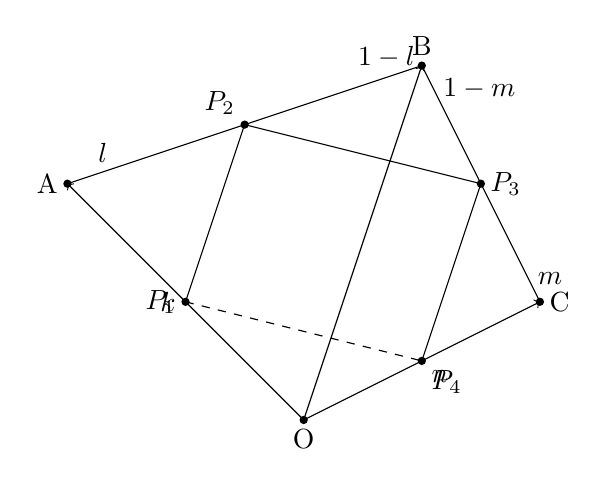
\begin{tikzpicture}[scale=1.5]
\coordinate (O) at (0,0);
\coordinate (A) at (-2,2);
\coordinate (B) at (1,3);
\coordinate (C) at (2,1);

\coordinate (P1) at (-1,1);
\coordinate (P2) at (-0.5,2.5);
\coordinate (P3) at (1.5,2);
\coordinate (P4) at (1,0.5);

\draw[->] (O) -- (A) node[midway, left] {$k$};
\draw[->] (O) -- (B);
\draw[->] (O) -- (C) node[midway, below right] {$n$};

\draw (A) -- (B) node[pos=0.1, above] {$l$} node[pos=0.9, above] {$1-l$};
\draw (B) -- (C) node[pos=0.1, right] {$1-m$} node[pos=0.9, right] {$m$};

\fill (O) circle (1pt) node[below] {O};
\fill (A) circle (1pt) node[left] {A};
\fill (B) circle (1pt) node[above] {B};
\fill (C) circle (1pt) node[right] {C};

\fill (P1) circle (1pt) node[left] {$P_1$};
\fill (P2) circle (1pt) node[above left] {$P_2$};
\fill (P3) circle (1pt) node[right] {$P_3$};
\fill (P4) circle (1pt) node[below right] {$P_4$};

\draw (P1) -- (P2) -- (P3) -- (P4);
\draw[dashed] (P1) -- (P4);
\end{tikzpicture}
\end{center}

\subsection*{第3問}
[解] $f(x) = k(x^{m+1}-1) - (x^m-1)$ とおく。$f(x) \ge 0$ が $0 < x$ の任意の$x$で成り立つ$k$の条件をしらべる
\begin{align*}
f'(x) &= k(m+1)x^m - mx^{m-1} \\
&= \{k(m+1)x - m\} x^{m-1}
\end{align*}
から、下表を得る

\begin{center}
\begin{tabular}{|c|c|c|c|c|}
\hline
$x$ & $0$ & $\cdots$ & $\frac{m}{k(m+1)}$ & $\cdots$ \\ \hline
$f'$ & & $-$ & $0$ & $+$ \\ \hline
$f$ & & $\searrow$ & & $\nearrow$ \\ \hline
\end{tabular}
\end{center}

よって、
\begin{align*}
f(x) &\ge f\left(\frac{m}{k(m+1)}\right) = k \left[ \left\{\frac{m}{k(m+1)}\right\}^{m+1} - 1 \right] - \left[ \left\{\frac{m}{k(m+1)}\right\}^m - 1 \right] \\
&= \left\{\frac{m}{k(m+1)}\right\}^m \left( \frac{m}{m+1} - 1 \right) + (1-k) \cdots \text{①}
\end{align*}

$x \to \infty$ とすれば、$k > 0$ が必要なので、$t = \frac{1}{k}$ とおいて、①を$g(t)$とすると
\[ g(t) = - \frac{m^m}{(m+1)^{m+1}} t^m + 1 - \frac{1}{t} \]
\[ g'(t) = - \frac{m^{m+1}}{(m+1)^{m+1}} t^{m-1} + \frac{1}{t^2} \]
より、下表をえる

\begin{center}
\begin{tabular}{|c|c|c|c|c|}
\hline
$t$ & $0$ & $\cdots$ & $\frac{m+1}{m}$ & $\cdots$ \\ \hline
$g'$ & & $+$ & $0$ & $-$ \\ \hline
$g$ & & $\nearrow$ & & $\searrow$ \\ \hline
\end{tabular}
\end{center}

これから
\[ g(t) \le g\left(\frac{m+1}{m}\right) = 0 \]
だから、常に $f(x) \ge 0$ がみたされるには、$t = \frac{m+1}{m} \Leftrightarrow k = \frac{m}{m+1}$ が条件である。

\subsection*{第4問}
[解] (1) $PQ = x, QS = y, QR = z$ (いずれも正) とおくと、
ピタゴラスから
\[ \begin{cases} a^2 = x^2 + y^2 \\ a^2 = x^2 + z^2 \end{cases} \cdots \text{①} \]
だから、四面体の体積$V$として
\[ V = \frac{1}{6}xyz = \frac{1}{6}x(a^2-x^2) \quad (\because \text{①}) \quad (0 < x < a) \]
\[ \frac{d}{dx}V = \frac{1}{6}(a^2-3x^2) \]
から下表をえる

\begin{center}
\begin{tabular}{|c|c|c|c|c|}
\hline
$x$ & $0$ & $\cdots$ & $\frac{\sqrt{3}}{3}a$ & $a$ \\ \hline
$V'$ & & $+$ & $0$ & $-$ \\ \hline
$V$ & & $\nearrow$ & & $\searrow$ \\ \hline
\end{tabular}
\end{center}

よって、$\max V$ は $x = \frac{\sqrt{3}}{3}a$ のときの $\frac{\sqrt{3}}{27}a^3$

\begin{center}
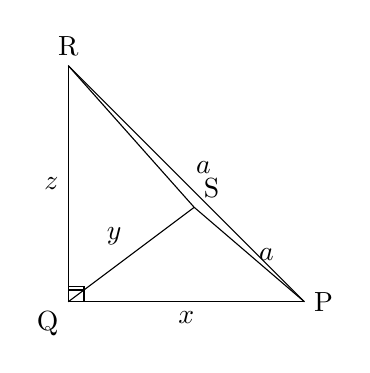
\begin{tikzpicture}[scale=2]
\coordinate (Q) at (0,0);
\coordinate (P) at (1.5,0);
\coordinate (R) at (0,1.5);
\coordinate (S) at (0.8,0.6);

\draw (Q) -- (P) node[midway, below] {$x$};
\draw (Q) -- (R) node[midway, left] {$z$};
\draw (Q) -- (S) node[midway, above left] {$y$};
\draw (P) -- (S) node[midway, right] {$a$};
\draw (P) -- (R) node[midway, above right] {$a$};
\draw (S) -- (R);

\node[below left] at (Q) {Q};
\node[right] at (P) {P};
\node[above] at (R) {R};
\node[above right] at (S) {S};

\draw (0.1,0) -- (0.1,0.1) -- (0,0.1);
\draw (0.1,0) -- (0.1,0.075) -- (0,0.075);
\end{tikzpicture}
\end{center}

(2) $AC$の中点$M$とする。対称性から $AC \perp MB, AC \perp DM$ であり、四面体$ABCD$の体積$V$、四面体$ABDM$の体積$V'$として
\[ V = 2V' \cdots \text{②} \]
である。面$\triangle ABM$を固定して $\angle BMD = \alpha \ (0 < \alpha < \pi)$ をうごかすと底面積を考えて$V'$は
$\alpha = \frac{\pi}{2}$ で$\max$である。この時の体積は(1)から $\frac{\sqrt{3}}{27}a^3$ だから ②に代入
\[ V = \frac{2\sqrt{3}}{27}a^3 \]

\begin{center}
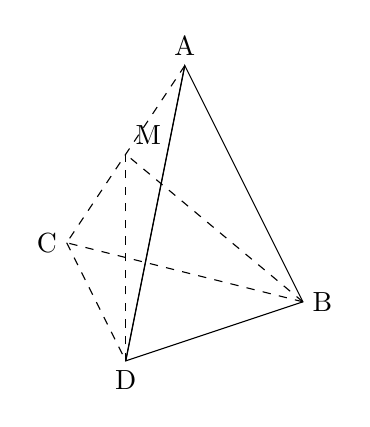
\begin{tikzpicture}[scale=1.5]
\coordinate (A) at (0,2);
\coordinate (B) at (1,0);
\coordinate (C) at (-1,0.5);
\coordinate (D) at (-0.5,-0.5);
\coordinate (M) at (-0.5, 1.25);

\draw (A) -- (B) -- (D) -- cycle;
\draw (A) -- (D);
\draw[dashed] (A) -- (C);
\draw[dashed] (B) -- (C);
\draw[dashed] (C) -- (D);
\draw[dashed] (B) -- (M);
\draw[dashed] (D) -- (M);

\node[above] at (A) {A};
\node[right] at (B) {B};
\node[left] at (C) {C};
\node[below] at (D) {D};
\node[above right] at (M) {M};
\end{tikzpicture}
\end{center}

\begin{center}
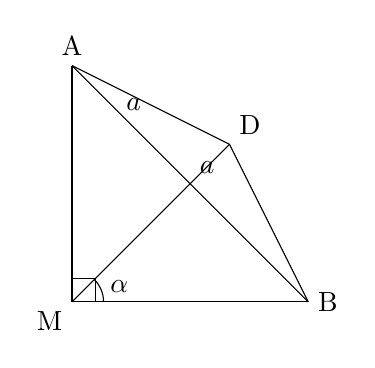
\begin{tikzpicture}[scale=2]
\coordinate (M) at (0,0);
\coordinate (A) at (0,1.5);
\coordinate (B) at (1.5,0);
\coordinate (D) at (1,1);

\draw (M) -- (A);
\draw (M) -- (B);
\draw (M) -- (D);
\draw (A) -- (B) node[midway, above right] {$a$};
\draw (A) -- (D) node[midway, left] {$a$};
\draw (B) -- (D);

\node[below left] at (M) {M};
\node[above] at (A) {A};
\node[right] at (B) {B};
\node[above right] at (D) {D};

\draw (0.2,0) arc (0:45:0.2);
\node at (0.3,0.1) {$\alpha$};
\draw (0,0.15) -- (0.15,0.15) -- (0.15,0);
\end{tikzpicture}
\end{center}

\subsection*{第5問}
[解] $k$ ($1 \le k \le N-1$) 回目に大吉を引く確率$p_k$は
\[ p_k = (1-p)^{k-1}p \]
$N$回目のおみくじを引く確率は
\[ p_N = (1-p)^{N-1} \]
だから
\begin{align*}
E &= \sum_{k=1}^N k p_k \\
&= \sum_{k=1}^{N-1} pk(1-p)^{k-1} + N(1-p)^{N-1} \cdots \text{①}
\end{align*}
であり
\[ \begin{cases} \frac{S}{p} = 1 + 2(1-p) + \cdots + (N-1)(1-p)^{N-2} \\ (1-p)\frac{S}{p} = (1-p) + \cdots + (N-2)(1-p)^{N-2} + (N-1)(1-p)^{N-1} \end{cases} \]
から辺々引いて
\begin{align*}
S &= \sum_{k=0}^{N-2} (1-p)^k - (N-1)(1-p)^{N-1} \\
&= \frac{1-(1-p)^{N-1}}{1-(1-p)} - (N-1)(1-p)^{N-1}
\end{align*}
だから①に代入して
\begin{align*}
E &= \frac{1-(1-p)^{N-1}}{p} - (N-1)(1-p)^{N-1} + N(1-p)^{N-1} \\
&= \frac{1-(1-p)^{N-1}}{p} + (1-p)^{N-1} \\
&= \frac{1-(1-p)^N}{p} \quad \text{(答)}
\end{align*}
であり、$(p, N) = \left(\frac{1}{5}, 10\right)$ の時
\begin{align*}
E &= 5 \left\{ 1 - \left(\frac{4}{5}\right)^{10} \right\} \\
&= 5 \left[ 1 - \left(\frac{8^5}{10^5}\right)^2 \right] \\
&\fallingdotseq 5 ( 1 - 0.107374 ) \cdots \bigstar \\
&= 4.463 \\
&\fallingdotseq 4.46 \quad \text{(答)}
\end{align*}

\subsection*{第6問}
[解1] (1) $0 < a \le x$ とする。部分積分から、
\begin{align*}
\int_a^x e^{-\frac{t^2}{2}} dt &= \int_a^x \frac{1}{t} \cdot t e^{-\frac{t^2}{2}} dt \\
&= \left[ \frac{1}{t} (-e^{-\frac{t^2}{2}}) \right]_a^x - \int_a^x \frac{1}{t^2} e^{-\frac{t^2}{2}} dt \\
&\le \frac{1}{a} e^{-\frac{a^2}{2}} - \frac{1}{x} e^{-\frac{x^2}{2}} \quad \text{(答)} \quad \left(\because \frac{1}{t^2} e^{-\frac{t^2}{2}} > 0, \text{等号成立は } x=a\right)
\end{align*}

(2)
\begin{align*}
\int_3^b e^{-\frac{t^2}{2} + 2t} dt &= \int_3^b \frac{1}{-t+2} (-t+2) e^{-\frac{t^2}{2} + 2t} dt \\
&= \left[ \frac{1}{-t+2} e^{-\frac{t^2}{2} + 2t} \right]_3^b - \int_3^b \frac{1}{(-t+2)^2} e^{-\frac{t^2}{2} + 2t} dt \\
&< e^{\frac{3}{2}} + \frac{1}{2-b} e^{-\frac{b^2}{2} + 2b} \quad \left(\because \frac{e^{-\frac{t^2}{2} + 2t}}{(-t+2)^2} > 0\right) \\
&< e^{\frac{3}{2}} \quad \text{(答)} \quad \left(\because \frac{1}{2-b} e^{-\frac{b^2}{2} + 2b} < 0\right)
\end{align*}

[解2] (1) $f(x) = \frac{1}{a} e^{-\frac{a^2}{2}} - \frac{1}{x} e^{-\frac{x^2}{2}} - \int_a^x e^{-\frac{t^2}{2}} dt$ とおく。
\[ f'(x) = \frac{1}{x^2} e^{-\frac{x^2}{2}} > 0 \]
及び $f(a) = 0$ から、$a \le x$ に対して $f(x) \ge f(a)$ である。 (答)

(2)
\end{document}
